\documentclass[a4paper,12pt]{article}

\usepackage[russian]{babel}
\usepackage{cmap}
\usepackage[utf8]{inputenc}
\usepackage[usenames]{color}
\usepackage{tabularray}
\usepackage{xcolor}
\usepackage{graphicx} 
\usepackage{subfigure}
\usepackage{subcaption}

\usepackage[unicode]{hyperref} % цвета гиперссылок
\hypersetup{
	colorlinks,
	citecolor=black,
	filecolor=black,
	linkcolor=blue,
	urlcolor=black
}

\usepackage{geometry} % задаёт поля 
%\geometry{left=3cm}
%\geometry{right= 1.5cm}
%\geometry{top=2cm}
%\geometry{bottom=2cm} 

\usepackage{enumitem} % настраивает работу со списками:
\def\labelitemi{—} % ... задаёт длинное тире как стандартный маркер ненумерованного списка
\setlist{nolistsep} %  ... убирает дополнительный отступы между элементами списка


% удаляет названия и продолжение следует и т. для таблиц, будет только таблица без всего
\DefTblrTemplate{contfoot-text}{default}{}
\DefTblrTemplate{conthead-text}{default}{}
\DefTblrTemplate{caption}{default}{}
\DefTblrTemplate{conthead}{default}{}
\DefTblrTemplate{capcont}{default}{}


\title{Сезонная структура потребления контента }
\author{В. Г. Мосин}
\date{}

%   \input{preamble.tex}
\begin{document}
	\maketitle
	\abstract{\noindent В статье исследована структура потребления образовательного контента в зависимости от сезона. Показано, что структура потребления в сезон высокого потребления отличается от структуры потребления в сезон низкого потребления. Рассмотрены регрессионные модели прогноза потребления. Показано, что модели, обученные на сезонах низкого потребления, хорошо подходят для прогнозов в сезон высокого потребления, причем, обратное не верно.}
	
\tableofcontents
	
\section{Введение}
Факторы сезонности в потреблении контента могут быть разнообразными и варьируются в зависимости от типа контента и предпочтений аудитории. Например, времена года, в которые проходят праздники, такие как Рождество, Новый год, День Святого Валентина, Хэллоуин и т. д., часто связаны с увеличенным интересом к праздничному контенту. Специфические сезонные мероприятия и события, такие как спортивные чемпионаты, фестивали или конференции, так же могут вызывать повышенный интерес и активность аудитории. Учитывая факторы сезонности, можно более эффективно адаптировать свои стратегии, выпуская соответствующий контент в нужное время для максимизации его востребованности (см. [5], [6]). 

В нашей работе мы будем изучать сезонную структуру потребления образовательного контента, в котором сезонные колебания интереса аудитории выражены особенно ярко (см. [8]). Учебные заведения работают по семестровой системе, и это оказывает сильное влияние на пики и спады потребления образовательного контента, так как во время семестров и активных периодов учебы спрос на образовательный контент значительно выше, в то время как в периоды каникул спрос минимален.

\subsection{Теоретическая часть}

Итак, есть сезоны высокого потребления образовательного контента, и есть сезоны низкого потребления. Мы будем изучать различия и сходства в сезонной структуре его потребления, используя регрессионный анализ — один из хорошо известных инструментов прогнозирования (см. [3], [4]). Он позволяет определить основные факторы и тенденции, влияющие на потребление, и прогнозировать его на будущее, основываясь на результатах предыдущих наблюдений. 

Однако в нашей работе, помимо прогнозирующих возможностей наших моделей, нас будет интересовать еще и структура моделей, так как именно она позволяет говорить о различиях или сходствах процессов потребления в разные сезоны. В регрессионной модели каждый предиктор имеет свой коэффициент, который показывает, как изменяется зависимая переменная при изменении значения предиктора (см. [3]). Если коэффициент значимый, то это означает, что предиктор оказывает статистически значимое влияние на зависимую переменную, если он близок к нулю, его влияние минимально. 

Оценивая не каждый коэффициент по отдельности, а всю их совокупность, можно судить о подобии структур потребления.

\subsection{Постановки задачи}

\subsubsection{Предмет исследования} Предметом исследования являются 10 наборов данных о потреблении контента информационного канала, относящегося к образовательной тематике. Данные образуют 2 группы по 5 наборов наблюдений в каждой группе. В одной группе представлены данные о потреблении контента в сезон высокого потребления (периоды зимней сессии, январи с 2019 по 2023), в другой — о потреблении в сезон низкого потребления (периоды летних каникул, августы с 2019 по 2023).

\subsubsection{Методика исследования} Методика состоит в обучении 10 регрессионных моделей на каждом из 10 наборов данных с последующим перекрестным тестированием по схеме «все на всех».

\subsubsection{Цель исследования} Наша цель состоит в описании структуры потребления контента, то есть, в указании значимых предикторов регрессионных моделей, и последующем сравнении структур высокого и низкого сезонов потребления. Кроме того, мы хотим выяснить, способны ли модели высокого и низкого сезонов прогнозировать друг друга на достаточном уровне точности прогнозов.

\subsection{Технологии}
Для выполнения вычислений и анализа данных мы пользуемся средой \texttt{Jupyter Notebook}, которая предоставляет удобные средства для работы с языком программирования Python и его главными библиотеками: \texttt{NumPy}, \texttt{Pandas}, \texttt{sklearn} и \texttt{matplotlib}. Благодаря этим инструментам, мы можем эффективно работать с данными, выполнять исследования и визуализировать результаты (см. [1], [2]).

Библиотека \texttt{numpy} является одной из ключевых библиотек для научных вычислений и обработки массивов данных в языке программирования \texttt{Python}. Она предлагает эффективные структуры данных, алгоритмы и функции для операций с многомерными числовыми массивами.

Библиотека \texttt{pandas}~--- одна из наиболее популярных и мощных библиотек для работы с данными в языке программирования \texttt{Python} (см. [1]). Она тесно взаимодействует с другими инструментами для вычислений и анализа данных на платформе \texttt{Python}, такими как \texttt{numpy}, \texttt{sklearn} и \texttt{matplotlib}. Это обеспечивает эффективную работу с информацией и применение различных алгоритмов и функций для анализа и визуализации данных.

Библиотека \texttt{scikit-learn}, широко известная как \texttt{sklearn}, предоставляет обширный набор инструментов и функций для решения различных задач в языке программирования Python, таких как задачи классификации, регрессии, кластеризации и др. Мы используем эту библиотеку для решения регрессионных задач.

\section{Описание данных}
Данные представляют собой набор из 10 сезонных отчетов о взаимодействии пользователей с контентом информационного канала на одном из ведущих хостингов. Наблюдения проводились в течение 5 лет, с 2019 по 2023 г., сезонная дифференциация осуществлялась по принципу: январь~--- сезон высокого потребления контента, август~--- сезон низкого потребления. Каждый из 10 отчетов содержит около 500 записей, точные значения объемов данных приведены ниже.

\section{Алгоритм}
\subsection{Чтение данных}
Методом \texttt{read\_csv} библиотеки \texttt{pandas} загружаем в среду исполнения 10 наборов данных (соответственно периодам наблюдений) и формируем 10 однотипных дата-фреймов. Таковы, например, данные за январь 2023:

\noindent
%---------------------------------------
%---------------------------------------
\SetTblrInner{rowsep=3pt}
%---------------------------------------
\begin{longtblr}
	{
		colspec = {
			X[r,f]
			X[r,f,4] 
			X[r,f,4] 
			X[r,f,4] 
			X[c,f,4]
			X[r,f,4]
		},
		width = \linewidth,
		rowhead = 1, 
		rowfoot = 0,
		row{odd} = {}, 
		row{even} = {},
		rows    = {font=\scriptsize},
		row{1}  = {font=\scriptsize\bfseries}
	}
	&
	Поделились 
	& 
	Просмотры
	&
	Показы 
	&
	...
	& 
	Время просмотра
	\\
	\hline[1pt]
	
	\textbf{0}   & 32.0   & 1892.0   & 5994.0   & ... & 94.7677 
	\\
	\hline
	\textbf{1}   & 1.0    & 362.0    & 2356.0   & ... & 15.0828 
	\\
	\hline
	\textbf{2}   & 0.0    & 45.0    & 668.0    & ...  & 1.6504 
	\\
	\hline
	\textbf{...} & ...    & ...     & ...      & ...  & ... 
	\\
	\hline
	\textbf{498} & 0.0    & 37.0    & 325.0    & ...  & 1.0950 
	\\
	\hline
	\textbf{499} & 0.0    & 6.0     & 70.0     & ...  & 0.2132 
	\\
	\hline[1pt]
\end{longtblr}
%---------------------------------------
\noindent
Каждая строка описывает определенный видеоролик, каждый столбец указывает на один из признаков, при помощи которого этот ролик описывается.  Применяем метод \texttt{describe} библиотеки \texttt{pandas} и выводим сведения о признаках. Для января 2023 они таковы:

\noindent
%---------------------------------------
\begin{longtblr}
	{
		colspec = {
			X[r,m, 3]
			X[r,m] 
			X[r,m] 
			X[r,m] 
			X[r,m]
		},
		width = \linewidth,
		rowhead = 1, 
		rowfoot = 0,
		row{odd} = {}, 
		row{even} = {},
		rows    = {font=\scriptsize},
		row{1}  = {font=\scriptsize\bfseries}
	}
	&
	mean 
	& 
	std
	&
	min 
	&
	max
	\\
	\hline[1pt]
	\textbf{Новые комментарии} & 0.048000 & 0.231956 & 0.000000 & 2.000000
	\\
	\hline
	\textbf{Поделились} & 0.522000 & 2.225178 & 0.000000 & 32.000000
	\\
	\hline
	\textbf{Отметки "Не нравится"} & 0.068000 & 0.368303 & 0.000000 & 5.000000
	\\
	\hline
	\textbf{Отметки "Нравится"} & 1.14000 & 3.26093 & 0.000000 & 38.000000
	\\
	\hline
	\textbf{Средний процент просмотра} & 33.024520 & 3.26093 & 0.960000 & 141.990000
	\\
	\hline
	\textbf{Просмотры} & 70.996000 & 184.063257 & 1.000000 & 2061.000000
	\\
	\hline
	\textbf{Время просмотра (часы)} & 2.746957 & 8.395691 & 0.000800 & 99.291900
	\\
	\hline
	\textbf{Показы} & 555.144000 & 843.541223 & 19.000000 & 9558.000000
	\\
	\hline
	\textbf{CTR для значков видео (\%)} & 4.528100 & 3.496724 & 0.000000 & 17.800000
	\\
	\hline[1pt]
\end{longtblr}
%---------------------------------------
\noindentПропущенных значений нет, все данные относятся к типу с плавающей запятой. Все наборы данных имеют одинаковую структуру, признаки всегда следуют в одном и том же порядке.

\subsection{Сравнение средних значений}
Пользуясь методом \texttt{describe} библиотеки \texttt{pandas}, выводим средние значения признаков по периодам наблюдений (признаки следуют в том же порядке, что и в таблице сведений о признаках, приведенной выше):
\noindent
%---------------------------------------
\begin{longtblr}
	{
		colspec = {
			X[r,m]
			X[r,m]
			X[r,m] 
			X[r,m] 
			X[r,m] 
			X[r,m] 
			X[r,m]
			X[r,m] 
			X[r,m] 
			X[r,m] 
			X[r,m]
		},
		width = \linewidth,
		rowhead = 1, 
		rowfoot = 0,
		row{odd} = {}, 
		row{even} = {},
		rows    = {font=\scriptsize},
		row{1}  = {font=\scriptsize\bfseries}
	}
	&
	01.19
	& 
	08.19
	
	&
	01.20
	& 
	08.20
	
	&
	01.21
	& 
	08.21
	
	&
	01.22
	& 
	08.22
	
	&
	01.23
	& 
	08.23
	
	\\
	\hline[1pt]
	{\textbf{1}}   
	& 0.68   & 0.01   & 0.08   & 0.01   & 0.09   & 0.02   & 0.06   & 0.03   & 0.04   & 0.01 
	\\
	\hline
	{\textbf{2}}          
	& 0.45   & 0.12   & 0.65   & 0.05   & 0.64   & 0.05   & 0.47   & 0.12   & 0.52   & 0.04
	\\
	\hline
	{\textbf{3}}          
	& 0.16   & 0.02   & 0.23   & 0.02   & 0.14   & 0.02   & 0.15   & 0.02   & 0.06   & 0.01
	\\
	\hline
	{\textbf{4}}          
	& 1.34   & 0.24   & 1.49   & 0.22   & 1.37   & 0.36   & 1.35   & 0.53   & 1.14   & 0.21
	\\
	\hline
	{\textbf{5}}          
	& 32.40   & 41.36   & 36.44   & 40.33   & 35.12   & 38.14   & 35.26   & 36.50   & 33.02   & 33.68
	\\
	\hline
	{\textbf{6}}
	& 96.89 &	16.54 &	100.35	& 17.51	   & 67.57	  & 14.18	 & 62.59  &	16.63	&  70.99	&  12.40          
	\\
	
	\hline
	{\textbf{7}}
    &4.43	&0.81	&4.50	&0.82	&2.82	&0.67	&2.81	&0.62	&2.74	&0.47          
	\\
	
	\hline
	{\textbf{8}}
    &778.74	&200.81	&903.22	&217.04	&780.09	&172.80	&486.05	&411.36	&555.14	&127.77        
	\\
	
	\hline
	{\textbf{9}}
    &3.88	&2.93	&3.56	&2.87	&3.14	&4.11	&4.23	&3.01	&4.52	&4.62
	\\
	
	\hline[1pt]
\end{longtblr}
%---------------------------------------
\noindent
Сравнивая средние значения по месяцам, делаем два наблюдения:
\medskip
\begin{enumerate}
	\item Январские значения почти всегда оказываются выше августовских, кроме двух показателей~--- 'Средний процент просмотра (\%)' и 'CTR для значков видео (\%)'~--- причем, оба эти показателя, в отличие от всех остальных, являются относительными, а не абсолютными.
	\item Значения некоторых показателей, например, 'Показы' и 'Новые комментарии', отличаются на порядки.
\end{enumerate}
\medskip
Отличие средних значений в пользу январских вполне естественно: мы изучаем структуру потребления образовательного контента, а август в образовании — это «мертвый сезон». Более того, основываясь именно на этом отличии, мы и проводим наше исследование. 

Что же касается существенного разброса значений, то это может привести к некорректным моделям, когда некоторые признаки будут получать преимущество просто из-за того, что их абсолютная величина перекрывает все остальные предикторы модели. Поэтому, прежде чем переходить к построению и сравнению регрессионных моделей, мы проводим нормализацию данных к стандартному виду с нулевым средним и единичной дисперсией.

\subsection{Нормализация данных}
В силу того, что данные были получены по отдельности друг от друга, в виде десяти самостоятельных дата-фреймов, нормализация на каждом из них была бы некорректной, так как средние значения всех показателей были бы нулевыми (см. [3]).
 
Для получения корректной нормализации, мы, пользуясь методом \texttt{concat} библиотеки \texttt{pandas}, производим конкатенацию данных в один дата-фрейм и только после этого нормализуем данные. Затем, пользуясь методом \texttt{loc}  для локализаций общего дата-фрейма, разбиваем его на фрагменты по периодам наблюдений, и, пользуясь методом \texttt{describe}, получаем нормализованные данные о средних значениях:
\noindent
%---------------------------------------
\begin{longtblr}
	{
		colspec = {
			X[r,m]
			X[r,m]
			X[r,m] 
			X[r,m] 
			X[r,m] 
			X[r,m] 
			X[r,m]
			X[r,m] 
			X[r,m] 
			X[r,m] 
			X[r,m]
		},
		width = \linewidth,
		rowhead = 1, 
		rowfoot = 0,
		row{odd} = {}, 
		row{even} = {},
		rows    = {font=\scriptsize},
		row{1}  = {font=\scriptsize\bfseries}
	}
	&
	01.19
	& 
	08.19
	
	&
	01.20
	& 
	08.20
	
	&
	01.21
	& 
	08.21
	
	&
	01.22
	& 
	08.22
	
	&
	01.23
	& 
	08.23
	
	\\
	\hline[1pt]
	{\textbf{1}}   
    &1.59	&–0.27	&–0.05	&–0.25	&–0.02	&–0.23	&–0.12	&–0.20	&–0.16	&–0.25
	\\
	\hline
	{\textbf{2}}          
    &0.09	&–0.13	&0.22	&–0.17	&0.22	&–0.17	&0.10	&–0.12	&0.13	&–0.18
	\\
	\hline
	{\textbf{3}}          
    &0.14	&–0.11	&0.28	&–0.11	&0.10	&–0.11	&0.11	&–0.12	&–0.03	&–0.14
	\\
	\hline
	{\textbf{4}}          
    &0.19	&–0.22	&0.25	&–0.23	&0.20	&–0.17	&0.20	&–0.11	&0.11	&–0.23
	\\
	\hline
	{\textbf{5}}          
    &–0.20	&0.27	&0.01	&0.22	&–0.05	&0.10	&–0.05	&0.01	&–0.17	&–0.13
	\\
	\hline
	{\textbf{6}}
    &0.37	&–0.23	&0.39	&–0.22	&0.15	&–0.25	&0.11	&–0.23	&0.17	&–0.26     
	\\
	
	\hline
	{\textbf{7}}
    &0.34	&–0.18	&0.35	&–0.18	&0.11	&–0.20	&0.10	&–0.21	&0.09	&–0.23        
	\\

	\hline
	{\textbf{8}}
    &0.36	&–0.30	&0.50	&–0.28	&0.36	&–0.33	&0.02	&–0.06	&0.10	&–0.38  
	\\
	
	\hline
	{\textbf{9}}
    &0.06	&–0.25	&–0.04	&–0.27	&–0.18	&0.13	&0.17	&–0.22	&0.27	&0.30
	\\
	
	\hline[1pt]
\end{longtblr}
%---------------------------------------
\noindent
Возвращаясь к сделанным выше наблюдениям, обнаруживаем:
\medskip
\begin{enumerate}
	\item Нормализованные средние значения январских показателей по-прежнему выше августовских (с теми же двумя исключениями).
	\item Разрыв в порядках наблюдаемых средних значений устранен, все значения относятся примерно к одному порядку.
\end{enumerate}
\medskip
Теперь, имея нормализованные данные, можно переходить к построению и обучению регрессионных моделей.

\subsection{Построение и обучение  моделей}

Мы будем строить десять моделей на десяти имеющихся у нас периодах наблюдений. В качестве целевой функции всегда будет выступать признак 'Время просмотра (часы)'.

\subsubsection{ Модель на данных за январь, 2019} 

Для получения левой части регрессионной задачи мы, пользуясь  методом \texttt{drop} библиотеки \texttt{pandas}, удаляем целевой признак 'Время просмотра (часы)' и переводим оставшийся дата-фрейм в массив \texttt{numpy}, пользуясь методом \texttt{to\_numpy}. В результате получается числовой массив X, содержащий  500 строк и 8 столбцов. Для получения правой части выделяем целевой признак, переводим его в массив и получаем одномерный числовой массив \texttt{y}, содержащий 500 элементов.

Затем, методом \texttt{LinearRegression} из модуля \texttt{linear\_model} библиотеки \texttt{sklearn}, мы формируем объект \texttt{model} и применяем к нему метод \texttt{fit} на массивах \texttt{X}, \texttt{y}.

\subsubsection{Модели на данных за другие периоды} 

Действуя точно так же, получаем и обучаем еще девять моделей.

\subsection{Коэффициенты регрессионных моделей}
Применяя метод \texttt{coef\_} библиотеки  \texttt{sklearn} к обученным выше моделям, выводим списки регрессионных коэффициентов и агрегируем их для сравнения:

\noindent
%---------------------------------------
\begin{longtblr}
	{
		colspec = {
			X[r,m]
			X[r,m]
			X[r,m] 
			X[r,m] 
			X[r,m] 
			X[r,m] 
			X[r,m]
			X[r,m] 
			X[r,m] 
			X[r,m] 
			X[r,m]
		},
		width = \linewidth,
		rowhead = 1, 
		rowfoot = 0,
		row{odd} = {}, 
		row{even} = {},
		rows    = {font=\scriptsize},
		row{1}  = {font=\scriptsize\bfseries}
	}
	&
	01.19
	& 
	08.19
	
	&
	01.20
	& 
	08.20
	
	&
	01.21
	& 
	08.21
	
	&
	01.22
	& 
	08.22
	
	&
	01.23
	& 
	08.23
	
	\\
	\hline[1pt]
	{\textbf{1}}   
    &–0.01	&0.11	&–0.09	&–0.02 	&0.00 	&0.07	&–0.03	&–0.02	&–0.01 	&0.00
	\\
	\hline
	{\textbf{2}}          
    &0.22 	&–0.03	&0.04	&0.01 	&0.10	&0.00	&0.06	&0.00	&0.18	&–0.01
	\\
	\hline
	{\textbf{3}}          
	&0.01	&–0.02	&–0.04	&0.06	&–0.04	&–0.02 	&–0.09	&0.03	&0.14  	&0.03
	\\
	\hline
	{\textbf{4}}          
    &0.15 	&0.09 	&0.22	&0.01 	&0.22	&0.05  	&0.02 	&0.03	&0.18 	&0.00
	\\
	\hline
	{\textbf{5}}          
    &0.06	&0.01 	&0.06 	&0.01 	&0.03	&0.01	&0.02	&0.01	&0.04	&0.01
	\\
	\hline
	{\textbf{6}}
    &0.91	&0.97	&0.72	&0.88	&0.67	&0.88	&1.01	&0.82	&0.38	&0.75
	\\
	
	\hline
	{\textbf{7}}
    &—	&—	&—	&—	&—	&—	&—	&—	&—	&—      
	\\
	
	\hline
	{\textbf{8}}
    &–0.08	&0.12	&0.19	&0.17	&–0.04	&0.09	&0.05	&–0.02	&0.19	&0.07 
	\\
	
	\hline
	{\textbf{9}}
    &–0.06	&–0.01	&–0.05	&–0.01	&–0.04	&0.00	&–0.05	&–0.01	&–0.02	&0.00
	\\
	
	\hline[1pt]
\end{longtblr}
%---------------------------------------
\noindent
В этой таблице мы сохранили седьмую строку 'Время просмотра (часы)', не придавая ей никаких значений, чтобы подчеркнуть, что этот признак является целевой функцией и не участвует в построении регрессионных моделей.

\subsection{Структура потребления контента}

Набор коэффициентов регрессионной модели является хорошей (хотя, и не единственной) иллюстрацией того, какова структура целевой функции: предикторы с более высокими коэффициентами вносят наибольших вклад в ее вычисление, предикторы с коэффициентами, близкими к нулю, несущественны. 

В нашем случае изучается структура потребления контента, которое мы естественным образом ассоциируем с общим временем просмотра, так как потребление видео~--- это и есть его просмотр. На иллюстрации (см. рис. 1) по горизонтали откладывается номер предиктора, а по вертикали~--- значение его коэффициента в регрессионной модели, то есть, то, насколько существенный вклад этот предиктор вносит в значение целевой функции.

\begin{figure}[!h]
	\centering
	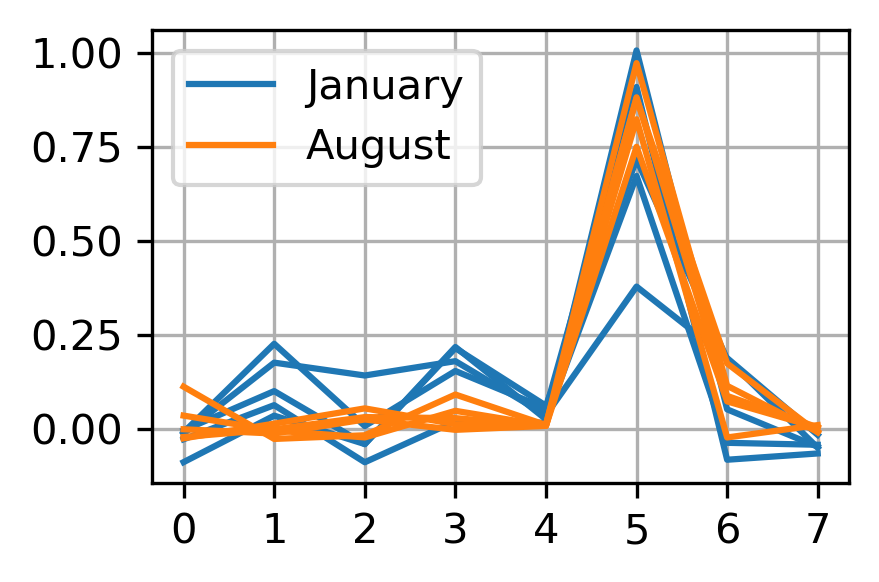
\includegraphics[width=0.4\linewidth]{pictures/Регрессионные коэффициенты по годам}
	\hspace{0.05\linewidth}
	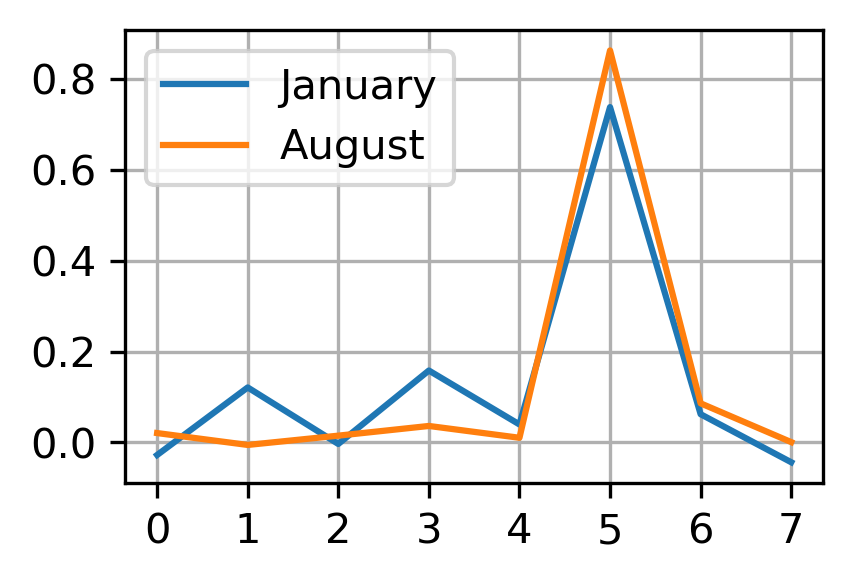
\includegraphics[width=0.4\linewidth]{pictures/Усредненные регрессионные коэффициенты}\\
	\caption{Структура потребления: (a) по годам, (b) усредненная}
\end{figure}

Наибольший коэффициент всегда относится к предиктору номер 5: это признак 'Просмотры', что совершенно не удивительно, так как количество просмотров сильно коррелирует с общим временем просмотра. Приоритет предиктора 'Просмотры' свойственен как январским, так и августовским моделям, и можно было бы сказать, что структура потребления контента сохраняется вне зависимости от сезона, но это не так.

После усреднения отчетливо видно, что январская модель обладает еще двумя приоритетами: это предиктор номер 1, 'Поделились', и предиктор номер 3, 'Отметки '{}'Нравится'{}'{}'. При этом усредненная августовская модель не считает их приоритетными. Следовательно, структура потребления на «низком» сезоне отличается от структуры «высокого» сезона, и это отличие еще проявит себя в процессе прогнозирования.

\subsection{3.8. Прогноз потребления контента}

У нас есть 10 обученных моделей: 5 январских и 5 августовских, и каждая из них дает свой прогноз потребления. С другой стороны, у нас есть 10 сезонов с реальными данными о потреблении контента: 5 январских и 5 августовских. Это дает нам возможность сопоставить прогнозируемые значения с реальными, то есть, оценить прогнозирующие способности моделей с разных точек зрения.

\subsubsection{Прогнозы модели, обученной на январе 2019} 
Сначала берем модель, обученную на январе 2019. Пользуясь методом \texttt{score} библиотеки \texttt{sklearn}, вычисляем коэффициент детерминации этой модели на данных за январь 2019 (в данном случае обучающая и тестовая выборки совпадают). Получаем $R^2 = 0.963$. Затем применяем эту модель к данным за январь 2020, получаем другой коэффициент детерминации: $R^2 = 0.899$. Оценка получилась ниже предыдущей. Это естественно, потому что в качестве обучающей выборки мы использовали данные за январь 2019, а в качестве тестовой~--- другие данные, за январь 2020. Затем применим модель к данным за январь 2021 и так далее. 

Таким образом, на этом шаге мы оцениваем прогнозирующую способность модели, обученной на январе 2019, для всех сезонов (включая сезон, на котором модель обучилась) и получаем 10 оценок.

\subsubsection{Прогнозы остальных моделей}

Действуем так же, как на предыдущем шаге: последовательно перебираем модели, обученные на остальных сезонах (их 9 шт.), применяем их ко всем сезонам (их 10 шт., включая сезон, на котором модель обучалась) и получаем еще 90 оценок.

\section{Результаты}

Метрики прогнозирующей эффективности для всех возможных попарных сезонных  прогнозов представлены в следующей матрице (в  ней по вертикали указаны сезоны, на которых обучалась модель, а по горизонтали — сезоны, на которых делался прогноз). 

\noindent
%---------------------------------------
\begin{longtblr}
	{
		colspec = {
			X[r,m]
			X[r,m]
			X[r,m] 
			X[r,m] 
			X[r,m] 
			X[r,m] 
			X[r,m]
			X[r,m] 
			X[r,m] 
			X[r,m] 
			X[r,m]
		},
		width = \linewidth,
		rowhead = 1, 
		rowfoot = 0,
		row{odd} = {}, 
		row{even} = {},
		rows    = {font=\scriptsize},
		row{1}  = {font=\scriptsize\bfseries}
	}
	&
	01.19
	& 
	01.20
	&
	01.21
	& 
	01.22	
	&
	01.23
	
	& 
	08.19
	&
	08.20
	& 
	08.21
	&
	08.22
	& 
	08.23
	
	\\
	\hline[1pt]
	{\textbf{01.19}}   
    &0.963	&0.899	&0.816	&0.917	&0.822	&0.815	&0.822	&0.676	&0.451	&0.158
	\\
	\hline
	{\textbf{01.20}}          
    &0.916	&0.961	&0.907	&0.943	&0.937	&0.725	&0.706	&0.244	&–1.301	&–1.061
	\\
	\hline
	{\textbf{01.21}}          
    &0.910	&0.929	&0.959	&0.939	&0.956	&0.804	&0.779	&0.760	&0.645	&0.484
	\\
	\hline
	{\textbf{01.22}}          
    &0.947	&0.946	&0.926	&0.960	&0.900	&0.876	&0.885	&0.784	&0.493	&0.460
	\\
	\hline
	{\textbf{01.23}}          
    &0.896	&0.918	&0.882	&0.933	&0.969	&0.770	&0.812	&0.701	&–1.408	&0.462
	\\
	\hline
	{\textbf{08.19}}
    &0.874	&0.892	&0.820	&0.916	&0.845	&0.952	&0.906	&0.888	&–1.035	&0.619
	\\
	
	\hline
	{\textbf{08.20}}
    &0.936	&0.916	&0.869	&0.942	&0.910	&0.914	&0.935	&0.899	&–0.932	&0.828  
	\\
	
	\hline
	{\textbf{08.21}}
    &0.929	&0.937	&0.920	&0.953	&0.925	&0.924	&0.918	&0.950	&0.080	&	0.845
	\\
	
	\hline
	{\textbf{08.22}}
    &0.895	&0.911	&0.934	&0.926	&0.949	&0.822	&0.856	&0.849	&0.887	&0.908
	\\
		
	\hline
	{\textbf{08.23}}
    &0.880	&0.907	&0.923	&0.917	&0.944	&0.833	&0.872	&0.892	&0.52	&0.925
	\\
	
	\hline[1pt]
\end{longtblr}
%---------------------------------------
\noindent
Матрица метрик обладает следующими свойствами:
\medskip
\begin{enumerate}
	\item На ее главной диагонали сосредоточены наибольшие значения. Это закономерно, так как в этих случаях модель тестируется на тех же данных, на которых она обучалась,  при этом коэффициент детерминации обладает заведомо большим значением.
	\item Она не симметрична. Например, модель, обученная на январе 2019 и примененная к январю 2020, и модель, обученная на январе 2020 и примененная к январю 2019~--- это две разные модели, и их коэффициенты детерминации различны: 
	$$R^2_{01.19 , 01.20} = 0.899 \ne 0.916 = R^2_{01.20 , 01.19}$$
	Неравенства имеют место и для всех остальных симметричных позиций.
	\item Самое удивительное свойство состоит в том, что модель, обученная на августовских данных, а протестированная на январских данных, всегда обладает большей прогнозирующей способностью, чем наоборот. Например, для августа 2019 мы можем сравнить первую половину строки 08.19 с первой половиной столбца 08.19:
	$$
	\begin{array}{c}
	R^2_{08.19 , 01.19} = 0.847 > 0.815 = R^2_{01.19 , 08.19}  \\
	R^2_{08.19 , 01.20} = 0.892 > 0.725 = R^2_{01.20 , 08.19}  \\
	R^2_{08.19 , 01.21} = 0.820 > 0.804 = R^2_{01.21 , 08.19}  \\
	R^2_{08.19 , 01.22} = 0.916 > 0.876 = R^2_{01.22 , 08.19}  \\
	R^2_{08.19 , 01.23} = 0.845 > 0.770 = R^2_{01.23 , 08.19}  \\
	\end{array}
	$$
	Соотношения остаются справедливыми для всех остальных августовских моделей, для этого достаточно рассмотреть другие пары полу-строк и полу-столбцов с номерами: 08.20, 08.21, 08.22, 08.23. Нет ни одного исключения.
	\item Матрица метрик не является блочной в алгебраическом понимании, но семантически она содержит 4 блока 5×5. Действительно:
	\begin{enumerate}
		\item Левый верхний блок описывает ситуации, когда модель обучается на январских данных и тестируется тоже на январских.
		\item Правый нижний блок~--- модель обучается на августовских данных и тестируется тоже на августовских.
		\item Правый верхний блок~--- модель обучается на январских  данных, а тестируется на августовских.
		\item Левый нижний блок~--- модель обучается на августовских данных, а тестируется на январских.
	\end{enumerate}
\end{enumerate}
\medskip
Усреднение коэффициентов детерминации по каждому из четырех блоков дает агрегированную по сезонам матрицу метрик:
\noindent
%---------------------------------------
%---------------------------------------
\SetTblrInner{rowsep=3pt}
%---------------------------------------
\begin{longtblr}
	{
		colspec = {
			X[r,f]
			X[r,f] 
			X[r,f] 
		},
		width = 0.4\linewidth,
		rowhead = 1, 
		rowfoot = 0,
		row{odd} = {}, 
		row{even} = {},
		rows    = {font=\scriptsize},
		row{1}  = {font=\scriptsize\bfseries}
	}
	&
	Январь 
	& 
	Август
	\\
	\hline[1pt]
	
	\textbf{Январь}   & 0.922   & 0.422
	\\
	
	\hline
	\textbf{Август}   & 0.911   & 0.682
	\\
	
	\hline[1pt]
\end{longtblr}
%---------------------------------------
\noindent
Ее содержательная интерпретация такова:
\medskip
\begin{enumerate}
	\item Наилучшие результаты получаются, когда модель, обученная на январских данных, применяется для прогнозирования к другим январским данным. 
	\item Модель, обученная на августе, в применении к другим августовским данным дает значительно худший результат. 
	\item Самая плохая ситуация возникает, когда модель, обученная на январе применяется к августовским данным. 
	\item И напротив: модель, обученная на августе, очень хорошо прогнозирует январские данные, лишь ненамного уступая моделям, которые учились на январе.
\end{enumerate}


\section{Выводы}
Эффект сезонности в потреблении образовательного контента означает, что объем потребления контента в образовании сильно меняется в зависимости от времени года, и это должно учитываться в анализе его потребления. Такой анализ помогает смоделировать и предсказать будущие сезонные колебания и адаптировать стратегии контент-провайдеров в соответствии с этими тенденциями (см. [7]).

\subsection{Обобщения}
Разумеется, сезоны высокого и низкого потребления имеют место не только в потреблении контента. Этот феномен широко распространен в различных сферах экономики и оказывает значительное влияние на бизнес-планы и стратегии компаний.
В сезоны высокого потребления входят периоды, когда спрос на товар или услугу возрастает до максимального уровня. Такие периоды могут быть связаны с различными факторами, включая сезонность (например, спрос на курорты и пляжные каникулы в летние месяцы), праздники (как Рождество или День святого Валентина), акционные мероприятия или повышенную активность в определенной отрасли. Сезоны низкого потребления, напротив, связаны с падением спроса до минимального уровня. 
Для компаний, работающих в условиях сезонности или колебания спроса, важно разрабатывать стратегии управления сезонами высокого и низкого потребления. Это тесно связано  с предсказанием поведения потребителей и разработкой маркетинговых акций, что, в свою очередь, требует моделирования и прогнозирования продаж.

\subsection{Моделирование на сезонах}
Результаты, изложенные нами в пункте 4 для потребления контента, естественным образом обобщаются на произвольное потребление, связанное с сезонным фактором. А именно: 
\medskip
\begin{enumerate}
	\item модель, обученная на сезоне высокого потребления, неприменима к сезону низкого потребления,
	\item и наоборот, модель, обученная на сезоне низкого потребления, показывает хорошие результаты как прогнозирующий инструмент для сезона высокого потребления.
\end{enumerate}
\medskip
Такой подход к прогнозированию потребления можно рекомендовать широкому кругу компаний, чья деятельность сопряжена с ярко выраженной сезонностью.

\section{Литература}
\begin{enumerate}
	\item Хейдт М. Изучаем Pandas / М. Хейдт~--- Москва: ДМК Пресс, 2018.~---438 с.
	\item Бурков А. Машинное обучение без лишних слов / А. Бурков~--- СПб: Питер, 2020.~--- 192 с.
	\item Вьюгин, В. В. Математические основы теории машинного обучения и прогнозирования / В. В. Вьюгин~--- М.: МЦИМО. — 2013.~--- 387~с.
	\item Бринк Х. Машинное обучение / Х. Бринк, Дж. Ричардс, М. Феверолф ~--- СПб.: Питер, 2017.~--- 336 с.
	\item Владимиров, В. А., Федорова, Ю. А. Моделирование сезонных колебаний в потреблении образовательного контента // Вестник Петербургского университета. Серия 5. Экономика. 2019. № 1. С.~82--93.
	\item Заяц, А. Л. Изучение и прогнозирование сезонности в потреблении образовательного контента на основе анализа временных рядов // Вестник Нижегородского университета имени Н. И. Лобачевского. Серия: Социальные науки. 2020. Т. 25. № 2 (2). С. 273--284.
	\item 7.Кашуба, А. Ю. Моделирование сезонной динамики в потреблении образовательного контента в условиях цифровизации // Молодой ученый. 2021. № 7 (335). С. 175--178.
	\item 8.Шустова, О. В., Ходьберг, Е. Н. Сезонность в потреблении образовательного контента: теория, моделирование, прогнозирование // Бизнес-информатика. 2021. Т. 15. № 3. С. 15--30.
\end{enumerate}






\end{document}